\subsection{Smovetec}
Bei dem Smovetec-System handelt es sich um eine Plattform, durch welche man Fahrradergometer horizontal beweglich machen kann. Dadurch kann man das Kurvenfahren mit einem echten Fahrrad sowie den Wiegetritt simulieren. Es eignet sich somit nicht nur für das übliche Konditionstraining, sondern auch zum Training von Balance und Geschicklichkeit.\\
Es können verschiedene Ergometer auf der Plattform festgeschraubt werden, wodurch man in der Wahl des Ergometers freigestellt ist.
\begin{figure}[ht]
\centering
\begin{subfigure}{.4\textwidth}
\centering
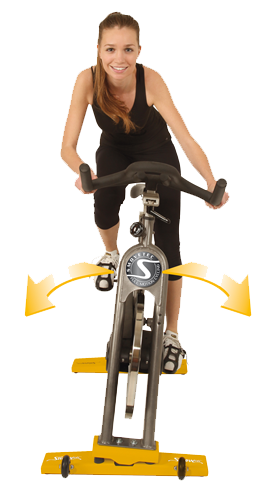
\includegraphics[width=.8\textwidth]{gfx/smovetec.png}
\caption{Das Smovetec-System im Einsatz}
\end{subfigure}
\begin{subfigure}{.59\textwidth}
\centering
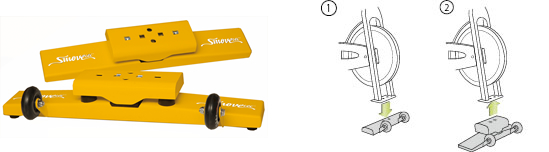
\includegraphics[width=.8\textwidth]{gfx/smovetec2.jpg}
\caption{Das Smovetec-System ohne Ergometer}
\end{subfigure}
\caption{Das Smovetec-System\footnotemark}
\end{figure}
\footnotetext{Quelle: \url{http://www.smovetec.de/smovetec-produkt.htm}}

\subsection{Texas Instruments SensorTag}
Das Smovetec-System selbst ist nicht mit Sensoren ausgestattet um Trittfrequenz oder Neigung zu messen. Um die Trittfrequenz zu messen, kommt in diesem Projekt ein \textit{SensorTag} der Firma Texas Instruments zum Einsatz. Hierbei handelt es sich um ein Bluetooth-fähiges Gerät, welches mit verschiedenen Sensoren ausgestattet ist. Diese umfassen:
\begin{itemize}
\item Temperatursensor
\item Feuchtigkeitssensor
\item Barometer
\item Beschleunigungssensor
\item Gyroskop
\item Magnetometer
\end{itemize}
Für unser Projekt wird davon ausschließlich der Beschleunigungssensor genutzt.\\
Um die Daten auszulesen, kommt eine erweiterte Version der Beispielapp von Texas Instruments zum Einsatz, welche insbesondere auch noch die Beschleunigungssensoren des Smartphones nutzt, um die Neigung zu erfassen. Die Daten werden vom Smartphone per WLAN weiter an den Rechner übermittelt, der das Spiel ausführt.
\begin{figure}[ht]
\centering
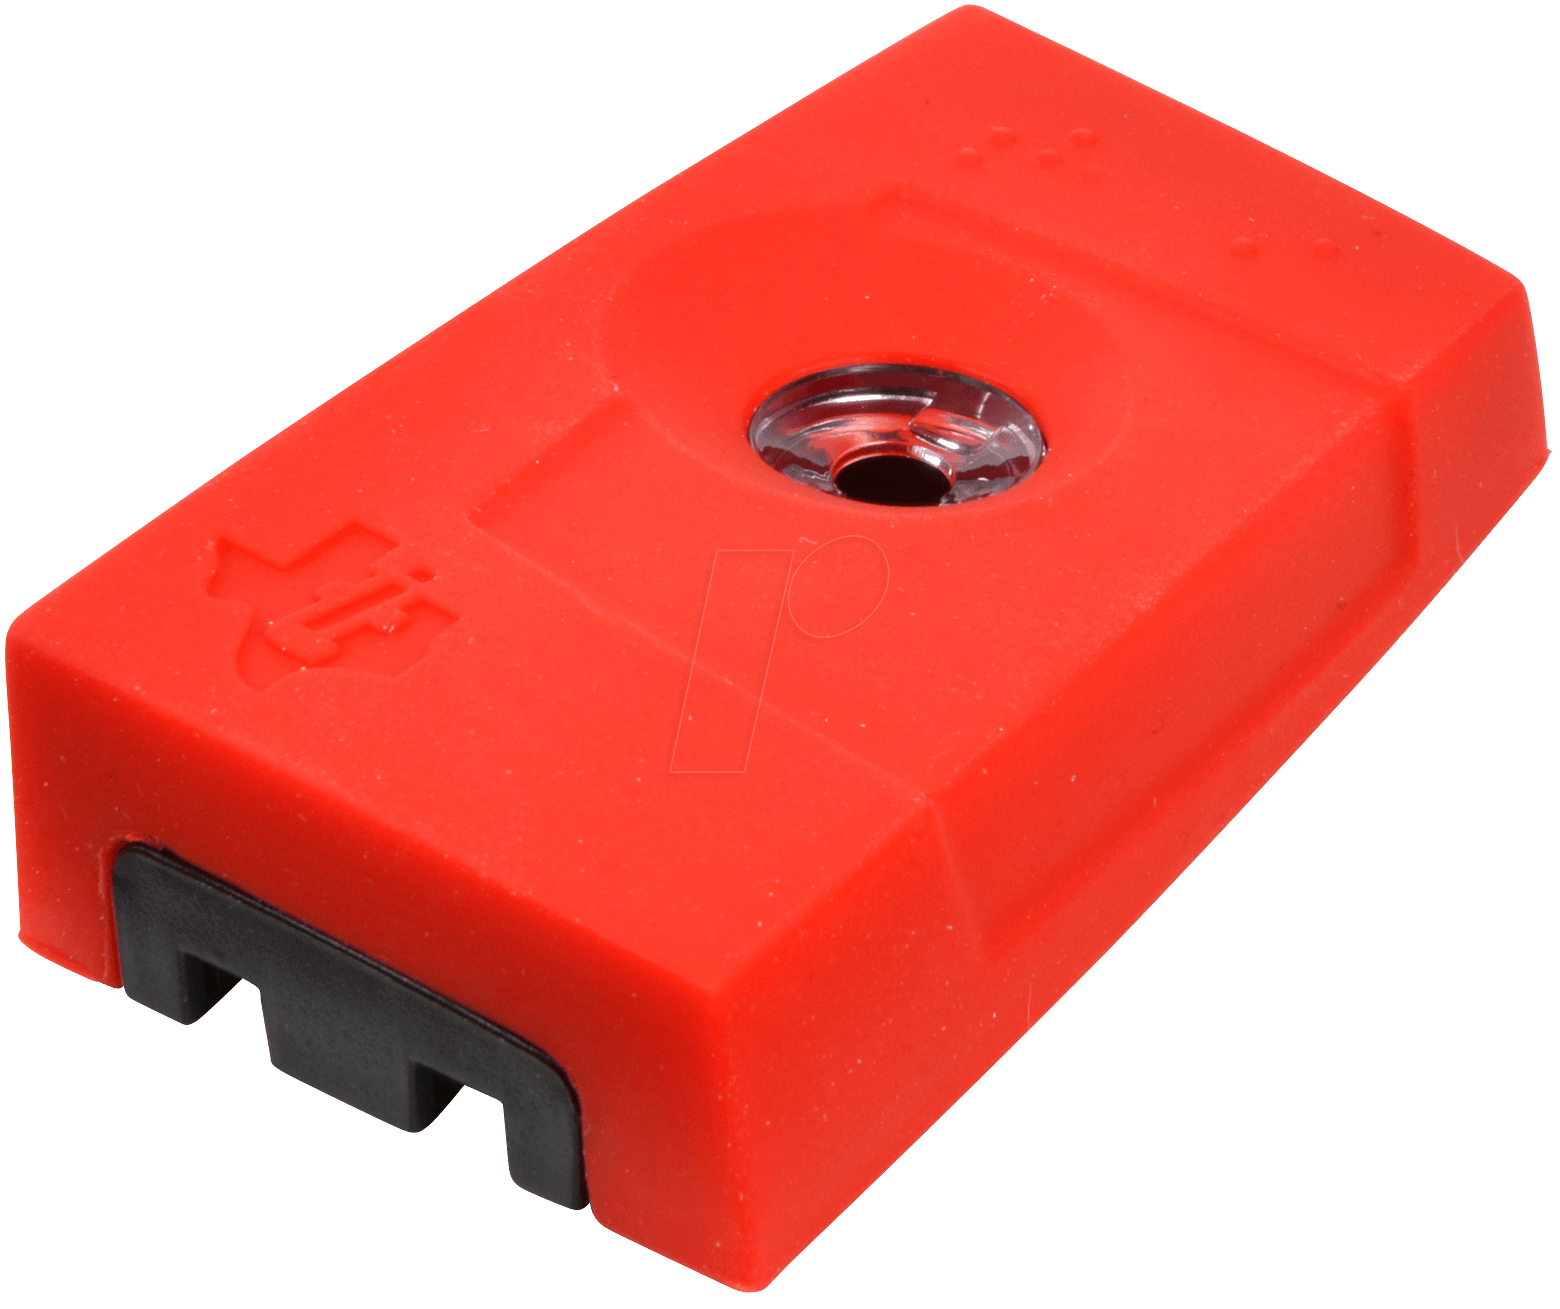
\includegraphics[width=.5\textwidth]{gfx/sensortag.png}
\caption{Texas Instruments SensorTag}
\end{figure}